\documentclass[../main.tex]{subfiles}

\begin{document}

\section{Materials and Methods}

\subsection{Microscopy}

A substantial amount of work for this project has been on determining the optimal microscopy technique for the live imaging of protein clustering.

The microscope used after trialling was as follows:

\begin{itemize}
\item{Nikon Eclipse Ti-E Inverted Microscope}
\item{40X 0.6NA long working distance plan objective}
\item{100X 1.49NA TIRF oil plan apo objective}
\item{Andor iXon 897 Ultra 512x512 pixel \SI{16}{\micro\meter} EMCCD camera}
\end{itemize}

\begin{figure}[h!]
\begin{center}
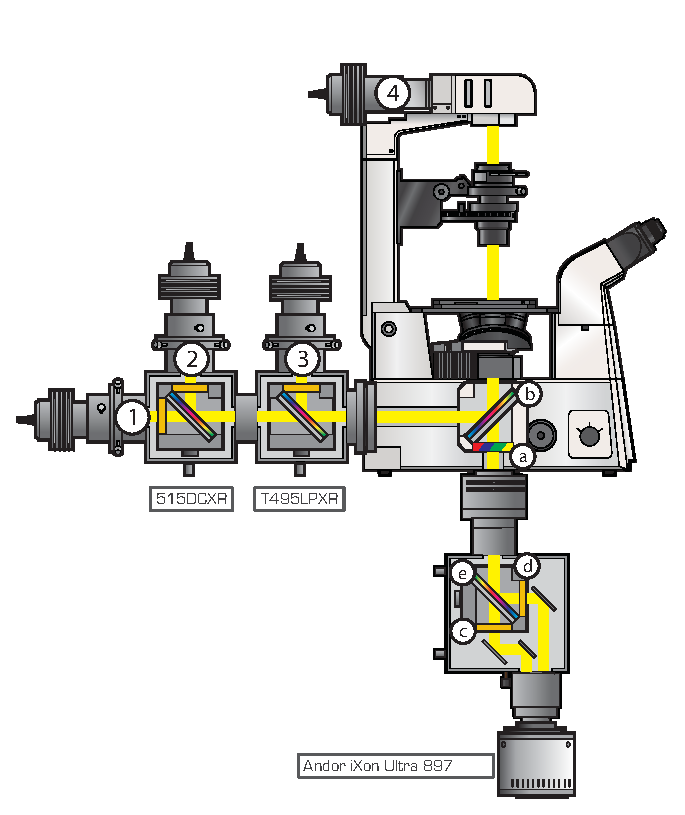
\includegraphics[scale=1]{\docroot matmeth/figs/microscope.eps}
\caption[Microscope schematic]{Microscope schematic. Whilst camera is shown on bottom port of microscope it is in fact mounted on left port. Numbered locations are for LED/filter combinations, given in Table~\ref{table:ledlighting}. Lettered locations are for emission filters or dichroics,  given in Table~\ref{table:filterset}.}
\label{fig:microscope}
\end{center}
\end{figure}

An OptoSplit II system from Cairn was employed to visualise both channels of Homo- or Hetero- FRET measurements simultaneously. This unit is placed in the lightpath between the microscope and the camera. Within it, a dichroic and pair of filters project the same half of the image onto each half of the camera sensor in different wavelengths or polarisation orientations. It is also possible to block one light path and allow the other to fully occupy the camera sensor by means of adjusting mirrors and shutters.

Inside the OptoSplit II is a dichroic and two filters (one in the case of anisotropy). Whilst there is already good wavelength filtering by the excitation and emission dichroics, the filters are required to clean up the signal and remove any longer wavelengths.

\paragraph{Excitation} was achieved with system described in Table~\ref{table:ledlighting}.
\begin{table}[h!]
\begin{center}
\begin{tabular}{l|c|c|l}
\textbf{Fluorophore}	&	\textbf{LED wavelength}	&	\textbf{Filter}	&	\textbf{Location} \\\hline
mCherry	&	White	&	560/40x	&	(1)	\\
YFP		&	\SI{505}{\nano\meter}		&	500/20x	&	(2)\\
GFP		&	\SI{470}{\nano\meter}		&	470/40x	&	(3)\\
Blue		&	White	&	440/10x	&	(3)\\
Bright Field		&	White	&	\SI{590}{\nano\meter}	&	(4)
\end{tabular}
\caption[LED lighting system]{LED lighting system for microscope. White LEDs comprised LED and phosphorescent elements. Excitation filter specifications give central wavelength and width of filter, both in \si{\nano\meter}, with the x denoting excitation. GFP and blue illumination sources are interchangeable.}
\label{table:ledlighting}
\end{center}
\end{table}

Only one blue (GFP or Blue) LED could be used at any one time. Lights from the back were combined sequentially with a \SI{515}{\nano\meter} and \SI{495}{\nano\meter} dichroic.

The white light for bright field has a red (\SI{590}{\nano\meter}) filter placed in front of it as the white LED requires a phosphorescent element to achieve the right spread of wavelengths. This phosphorescent element can be excited by fluorescence excitation, causing a high level of light to be reflected back through the lens and into the camera. The red filter blocks this transmission and allows for rapid switching between bright field and fluorescent excitation without having to block the light path.

For anisotropy measurements, a rotating linear polariser could be inserted in front of the YFP LED (position (2)).

The entire microscope is mounted on a ThorLabs PerformancePlus Series II breadboard fitted to a ThorLabs Active Isolation frame. This was felt necessary due to the presence of noisy machinery in adjacent rooms, high foot traffic, and small size of the samples being observed (\(\sim\)\SI{2.5}{\micro\meter} in the largest dimension).

\paragraph{Emission} was controlled with the filters described in Table~\ref{table:filterset}.
\begin{table}[h!]
\begin{center}
\begin{tabular}{l|c|c|c|c|c}
&	\multicolumn{2}{c|}{Filter Wheel}	&	\multicolumn{3}{c}{OptoSplit II}	\\
\textbf{Description}	&	\textbf{Dichroic} (b)	&	\textbf{Filter} (a)		& \textbf{Dichroic} (e)	&	\textbf{Filter} (d)	&	\textbf{Filter} (c)	\\\hline
mCherry	&	\SI{585}{\nano\meter}		&	630/75m	&	-	&	-	&	-	\\
YFP		&	\SI{515}{\nano\meter}		&	535/30m	&	-	&	-	&	-	\\
YFP Anisotropy	&	\SI{515}{\nano\meter}	&	535/30m	&	Polarising	&	Polarising	&	-	\\
YFP\(\rightarrow\)mCherry Fret	&	\SI{515}{\nano\meter}	&	-	&	\SI{565}{\nano\meter}	&	545/40m	&	630/75m	\\
GFP		&	\SI{495}{\nano\meter}		&	525/50m	&	-	&	-	&	-	\\
Bright field		&	-	&	-	&	-	&	-	&	-	
\end{tabular}
\caption[Microscope filter set]{Filter set. Emission filter specifications give central wavelength and width of filter, both in \si{\nano\meter}, with the m denoting emission.}
\label{table:filterset}
\end{center}
\end{table}


\subsection{Laboratory Techniques}

\subsubsection{Standard Protocols}
\paragraph{MiniPreps} were performed with either a Fermentas GeneJet kit (for sequencing) or boiling lysis protocol (for anything else).
\paragraph{PCR} was performed with Phusion\textregistered\xspace polymerase according to the following scheme:

\begin{center}
\begin{tabular}{lcc}
Initial Denaturation	& \SI{98}{\degreeCelsius} & \SI{120}{\second}\\
\multicolumn{3}{c}{\textbf{Loop 30 times:}}\\
Denaturation		&	\SI{98}{\degreeCelsius}		&	\SI{30}{\second}\\
Annealing 		&	Optimal for primer	&	\SI{30}{\second}\\
Extension		&	\SI{72}{\degreeCelsius}		&	\SI{30}{\second\per\kilo\base}\\
\multicolumn{3}{c}{\textbf{End Loop}}\\
Final extension	&	\SI{72}{\degreeCelsius}		&	\SI{7}{\minute}\\
Hold				&	\SI{4}{\degreeCelsius}		&	\(\infty\)
\end{tabular}
\end{center}

\paragraph{Transformation} was performed on \ce{CaCl} competent cells.

\subsubsection{Gibson Assembly}

Gibson Assembly can be performed in volumes from about \SIrange{5}{20}{\micro\litre}. Initially, larger volumes were used but as efficiency became apparent smaller volumes were used to economise. Roughly equimolar concentrations of gel purified overlapping DNA were added to the 1.33X Gibson Master Mix in a \SI{50}{\micro\litre} tube on ice. This was incubated for \SI{1}{\hour} at \SI{50}{\degreeCelsius}, before being returned to ice. \SIrange{5}{10}{\micro\litre} was then used to transform cells.

All protocols and buffers for Gibson Assembly are from~\citet{gibson09}.

\begin{table}
\begin{center}
\begin{tabular}{c|c|c}
&\textbf{Stock Concentration} (\si{\unit\per\micro\litre})&\textbf{Volume} (\si{\micro\litre})\\\hline
Taq ligase				&	40		&	50\\
5X Isothermal Buffer		&	5X		&	100\\
T5 Exonuclease			&	1		&	2\\
Phusion\textregistered\xspace Polymerase		&	2		&	6.25\\
Nuclease free water		&			&	216.75\\\hline
\textbf{Total}			&	1.33X	&	375
\end{tabular}
\caption[Gibson Master Mix]{Gibson Master Mix. This was prepared on ice in the Taq ligase tube, before being aliquoted into \SI{75}{\micro\litre} portions for freezing at \SI{-20}{\degreeCelsius}.}
\end{center}
\end{table}

\begin{table}
\begin{center}
\begin{tabular}{c|c|c}
&\textbf{Stock Concentration} (\si{\milli\Molar})&\textbf{Volume} (\si{\micro\litre})\\\hline
PEG-8000					&	25\%		&	\SI{0.75}{\gram}\\
Tris-\ce{HCl} pH 7.5		&	500		&	1500\\
\ce{MgCl2}				&	50		&	75\\
DTT						&	50		&	150\\
dATP						&	1		&	30\\
dTTP						&	1		&	30\\
dCTP						&	1		&	30\\
dGTP						&	1		&	30\\
NAD						&	5		&	300\\
Nuclease free water		&			&	...\\\hline
\textbf{Total}			&	5X		&	3000
\end{tabular}
\caption[5X Isothermal Buffer]{5X Isothermal Buffer. Prepared on ice and stored at \SI{-20}{\degreeCelsius}.}
\end{center}
\end{table}


\subsubsection{Preparation of Cells for Microscopy}

The following protocol was followed for preparing cells for microscopy.

\begin{enumerate}
\item Prepare \SI{2}{\milli\litre} overnight culture with appropriate antibiotic.
\item Pellet the cells in a \SI{1.5}{\milli\litre} microcentrifuge tube.
\item Aspirate off supernatant
\item \paragraph{If fixing}
\begin{enumerate}
\item Resuspend in \SI{500}{\micro\litre} PBS, with or without \ce{CoSO4}.
\item Add \SI{12.5}{\micro\litre} 37-41\% formaldehyde to make 1\%.
\item Incubate for 10 minutes at room temperature.
\end{enumerate}
\item \paragraph{If only adding cobalt}
\begin{enumerate}
\item Resuspend in \SI{500}{\micro\litre} PBS with \ce{CoSO4}.
\end{enumerate}
\item[] \paragraph{Then}
\item Spin down cells.
\item Resuspend in \SI{1}{\milli\litre} PBS.
\item Spin down cells.
\item Resuspend in \SI{500}{\micro\litre} PBS.
\end{enumerate}

The final resuspension volume was be adjusted to match cell density depending on mounting method. Initial volume was also be adjusted with corresponding changes to subsequent volumes. Concentration of \ce{CoSO4} was varied according to requirements.

\paragraph{STED} microscopy requires special cell preparation to help protect against bleaching. The following protocol was used from Jackson ImmunoResearch~\citep{jackson}:

\begin{enumerate}
\item Prepare and wash cells as above
\item Make up 90\% glycerol in 10X PBS
\item Make up 20\% w/v n-propyl gallate in dimethyl sulfoxide
\item Add 1/100 volume of 20\% NPG to 90\% glycerol/1x PBS dropwise with rapid stirring
\item Resuspend cells in \SI{500}{\micro\litre} of the above
\end{enumerate}

\paragraph{Cell Mounting} Cells were mounted on \#1.5 slides for imaging. Work is still ongoing to optimise a poly-L-lysine protocol to hold the cells in place.

\subsection{Image Processing}
\label{sec:methods:imageprocessing}
Unless otherwise stated, all image processing has been done in Matlab. All processing scripts are open source and have been made publicly available, see section~\ref{sec:scripts:clusters}.

\subsubsection{Cluster Detection}
One basic objective was to determine the size or protein density of the chemotaxis protein clusters on the poles of the \ecoli. At the start of the project there were existing scripts that identified clusters through threshold detection. Whilst this performed reasonably well on high contrast images, it struggled on more noisy images, and could not identify cells with more than one cluster, or none at all.

A brief description of the two scripts written to identify the size and density of clusters follows:

\paragraph{cell\_finder.m}\ \\
\texttt{[ cell\_mask, all\_cells, masks ] = cell\_finder( image, pixel\_size, search\_radius, minimum\_size, maximum\_size, eccentricity, solidity, max\_brightness ) }
\\\\
This function takes as its input the image of the cells, along with the following parameters:
\\\\
\begin{tabular}{rl}
Pixel Size		&	Length of pixel in microns\\
Search Radius 	&	Radius in which to search for cluster in microns\\
Minimum Size		&	Smallest cell size in square microns\\
Maximum Size		&	Largest cell size in square microns\\
Eccentricity		&	Minimum ratio of cell length to cell width\\
Solidity			&	Minimum solidity\\
Maximum Brightness	&	Maximum total brightness of cell
\end{tabular}
\\\\
The solidity gives a measure of the curvature of the cell. It measures the proportion of the convex hull of the cell that is occupied by the cell itself. If it is less than 0.8 then the cell is curved, or T-shaped, and thus not considered.

As its output the function gives an image mask to identify all cells identified as valid (\texttt{cell\_mask}), an image mask to identify all cells (\texttt{all\_cells}), and a series of other masks identifying all cells disqualified for being too small, large, round, bright, or not solid enough. This process is visualised in Figure~\ref{fig:imageprocessing:celldetection}.

\begin{figure}[p]
\begin{center}
\subfloat[Raw greyscale image]{
	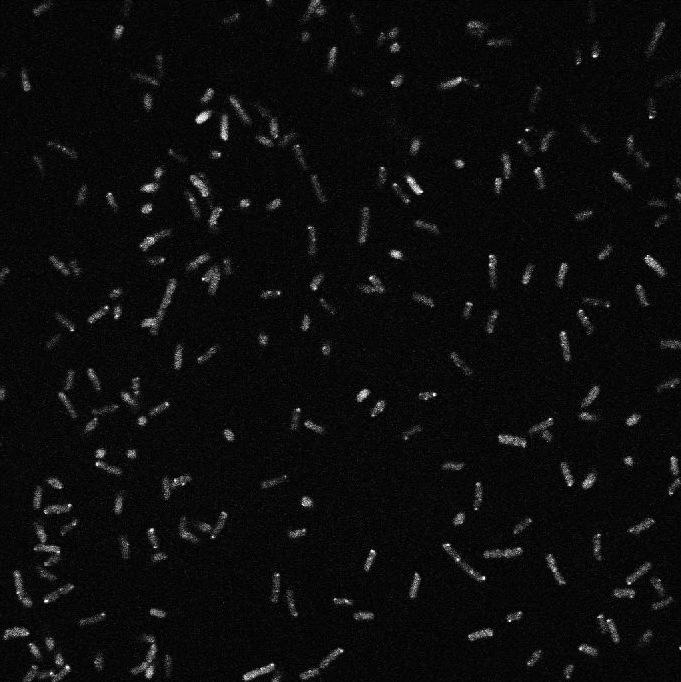
\includegraphics[scale=0.64]{\docroot matmeth/figs/slide1}
	\label{fig:imageprocessing:raw}
}
\subfloat[Edge detection]{
	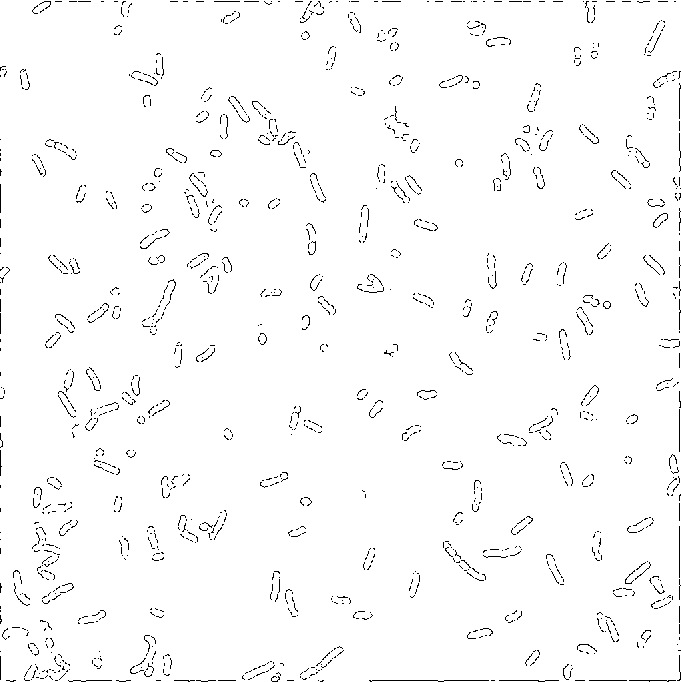
\includegraphics[scale=0.64]{\docroot matmeth/figs/slide2}
	\label{fig:imageprocessing:edges}
}\\
\subfloat[Detected Cells]{
	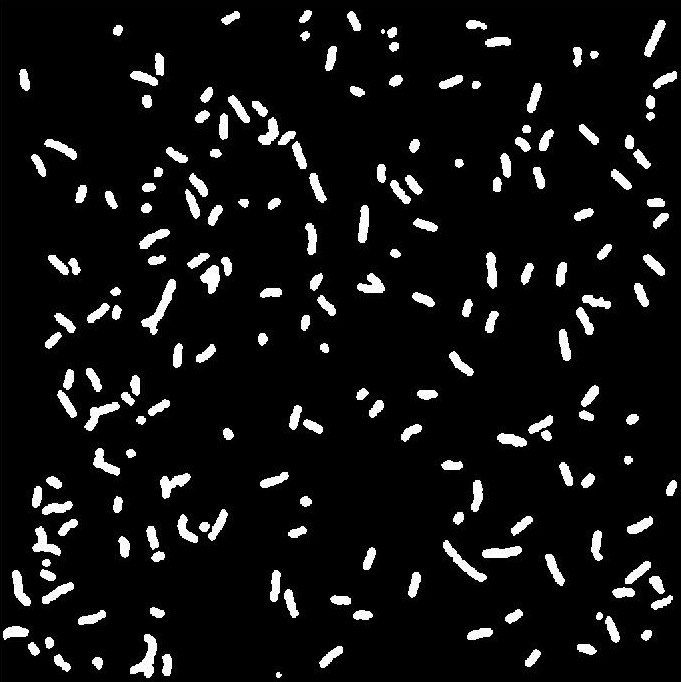
\includegraphics[scale=0.64]{\docroot matmeth/figs/slide3}
	\label{fig:imageprocessing:cells}
}
\subfloat[Accepted Cells]{
	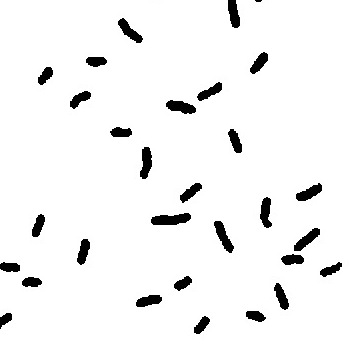
\includegraphics[scale=0.64]{\docroot matmeth/figs/slide4}
	\label{fig:imageprocessing:accepted}
}
\caption[Depiction of cell detection]{To generate the mask of cells, the script first performs edge detection using the Canny method~\citep{canny} (Figure~\subref{fig:imageprocessing:edges}). This is particularly effective for detecting edges in noisy images. The lines are then thickened and the gaps closed to give the outline of cells. These are filled in, and then the image is opened with a disk shaped element to remove any small blobs or bridges. This intermediate image is now \texttt{all\_cells} (Figure~\subref{fig:imageprocessing:cells}). Subsequently, each constraint on cell shape or size is applied individually to determine which cells to reject (Figure~\subref{fig:imageprocessing:accepted}). Images shown here have been cropped and inverted for clarity in print.}
\label{fig:imageprocessing:celldetection}
\end{center}
\end{figure}


\paragraph{cluster\_finder.m}\ \\
\texttt{[ cluster\_fraction, com\_pass, com\_fail ] = cluster\_finder( image, cell\_mask, all\_cells, pixel\_size, threshold, search\_radius, min\_cluster\_size, max\_cluster\_size ) }
\\\\
This function takes as its inputs the image of the cells, and the first two cell masks as described in the previous function. Along with these it takes the following parameters:
\\\\
\begin{tabular}{rl}
Pixel Size		&	Length of pixel in microns\\
Threshold		&	Minimum intensity for peak of cluster, relative to mean cell intensity\\
Search Radius 	&	Radius in which to search for cluster in microns\\
Minimum cluster size	&	Smallest radius of cluster in microns\\
Maximum cluster size	&	Maximum radius of cluster in microns
\end{tabular}
\\\\
As its output it provides a vector containing, for each cluster, the fraction of protein in the whole cell that was found in the cluster. It also contains two vectors containing the centres of mass of each identified cluster and each cluster that failed to meet the given constraints.

Before searching for clusters, the script subtracts low frequency background noise using a rolling ball average. The script then loops through each cell, trying to locate each cluster. Because the clusters are on the order of the resolution of the microscope (\SI{200}{\nano\meter}), they can be approximated as a 2D Gaussian. To do this, the script finds the brightest pixel not yet masked in the cell, and attempts to fit a 2D Gaussian curve using non-linear optimisation as shown in Figure~\ref{fig:imageprocessing:clusterdetection}, and masks off the surrounding area from further search. The 2D Gaussian curve is then used to approximate the proportion of fluorescent proteins detected within the cluster compared to the entire cell. This continues until no pixels brighter than the threshold can be found, and the script moves on to the next cell.

\begin{figure}[h!]
\begin{center}
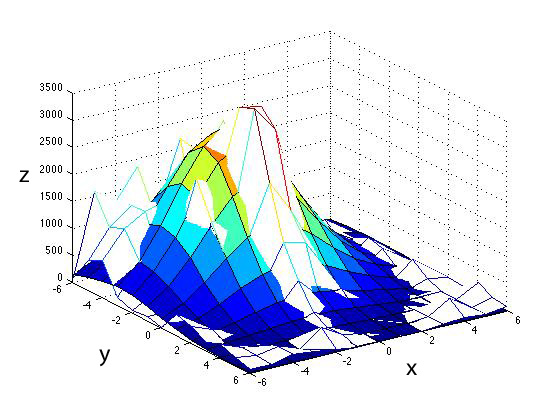
\includegraphics[scale=0.5]{\docroot matmeth/figs/slide5}
\caption[Depiction of cluster detection]{Depiction of cluster detection. X and Y axes are pixels, with the Z axis being the grey level of the image. The white surface with coloured lines is a plot of what the script thinks might be a cluster, and the coloured surface with black lines is a plot of the best fitting 2D gaussian.}
\label{fig:imageprocessing:clusterdetection}
\end{center}
\end{figure}



\subsubsection{Image Alignment}

The OptoSplit II provided by Cairn Research allows for viewing two channels on the same sensor simultaneously. However, as the two images are adjacent in the same file, they must be split into two separate aligned images so that they may be accurately overlaid. This can be automated using some fairly simple mathematical methods.

The two images are extracted with a \(\simeq10\%\) safety border. A mean is taken of each image in each of the x and y axes. A least-squares fitted straight line mean is subtracted from each to negate the effect of any gradient across the image. Each pair of means is then aligned by gradient descent of the root mean square of the difference between them.

This provides the six data points required to align all future images taken until the OptoSplit II is adjusted again - the size of the image, and both of the locations.

Again, all scripts are available online, see section~\ref{sec:scripts:anisotropy}.

\subsection{MicroManager}

In order to give maximum flexibility, the microscope and all related equipment were controlled using MicroManager~\citep{micromanager}, an open source software package for control of microscope and associated devices. A beanshell driver was written for the syringe pumps to allow easy integration into experimental workflow, along with several scripts to run experiments. Latest versions of these may be found online, see section~\ref{sec:scripts:micromanager}.

\end{document}
